%----------------------------------------------------------------------------
%----------------------------------------------------------------------------
%bb defines the bounding box for the pdf
%viewport defines the area of the pdf used
%in sidewaysfigure the last entry in bb moves the caption toward/away the pic
%in sidewaysfigure the second entry in bb moves the pic toward/away the caption
%----------------------------------------------------------------------------
\begin{figure}
\scalebox{0.8}[0.8]{
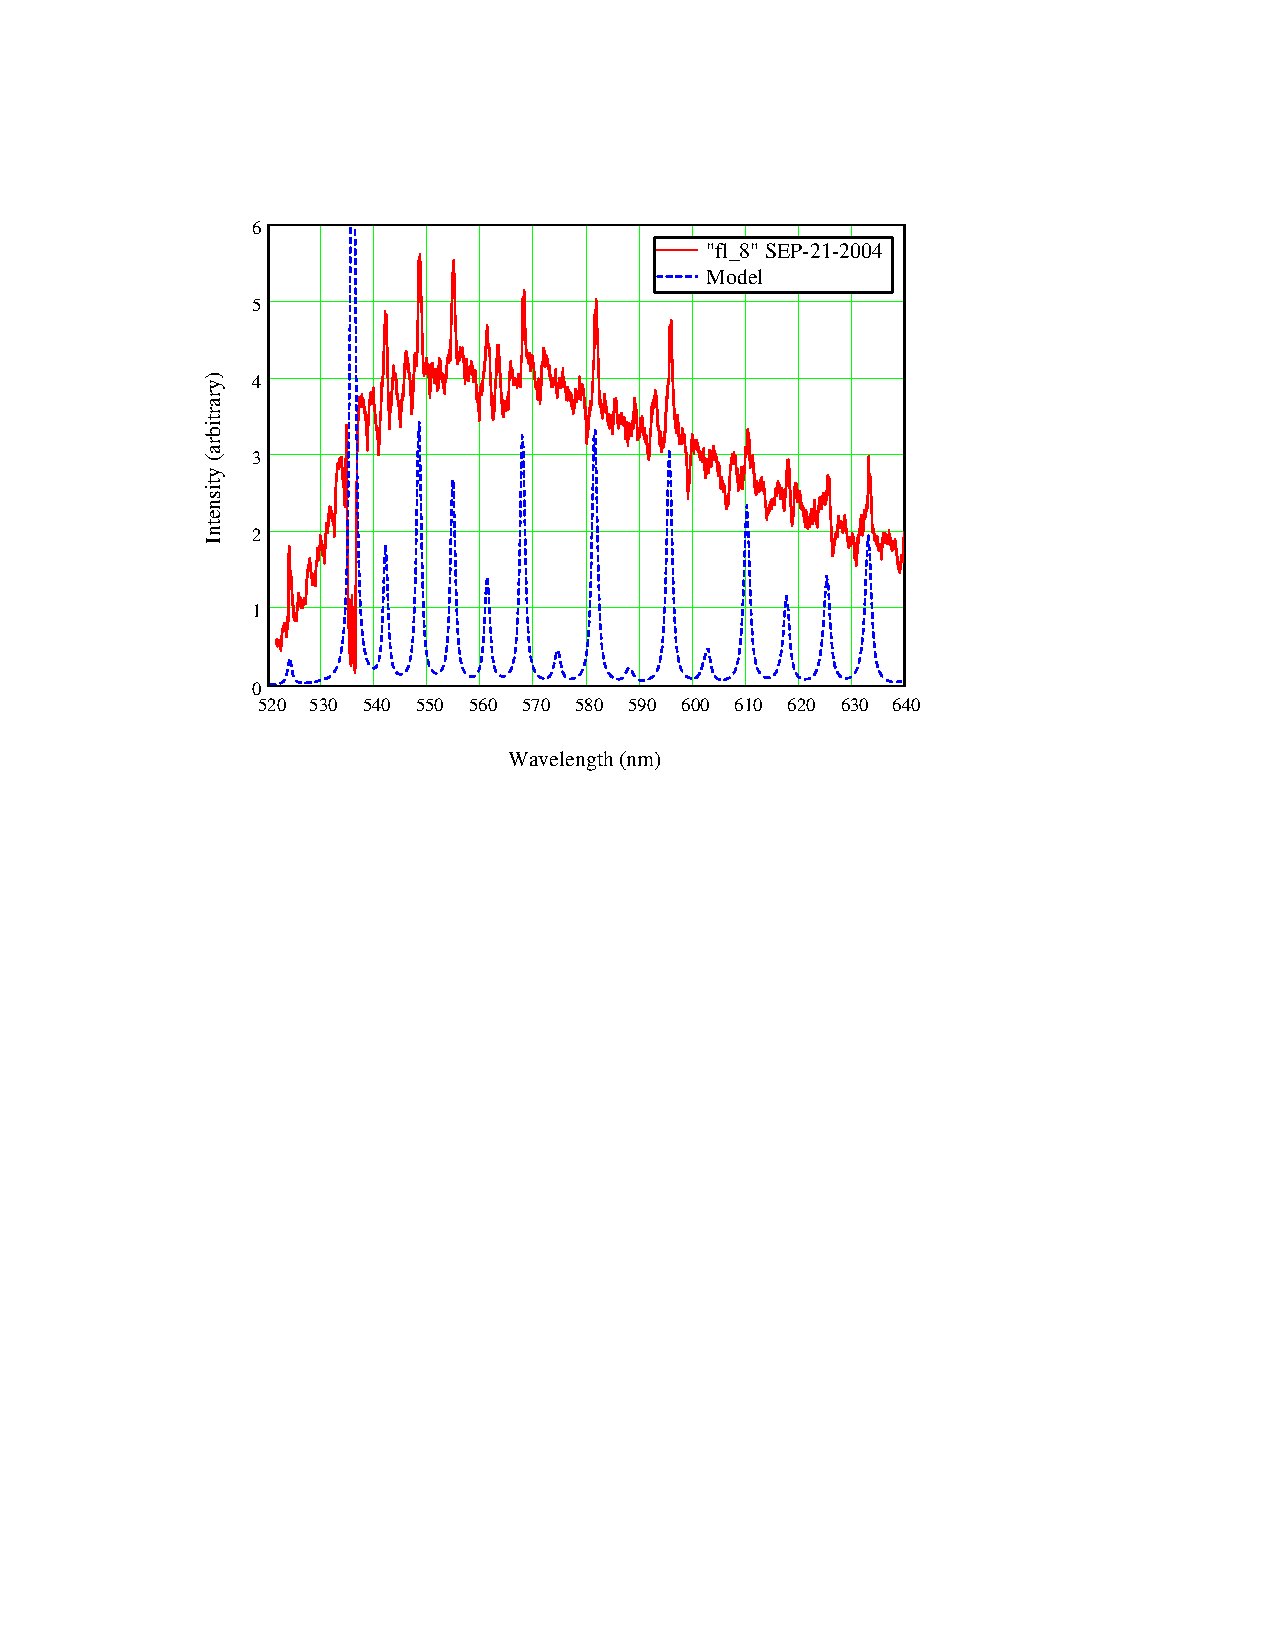
\includegraphics[bb=10 430 489 670]
{baked_potato/baked_potato.pdf}
}
\caption{535.8901 nm LIF from the ``baked potato'' iodine cell}
\label{baked_potato}
\end{figure}
%----------------------------------------------------------------------------

%----------------------------------------------------------------------------
While targeting transition two (see Section \ref{absorption data section}) with the dye laser (wavelength set at 535.8901 nm), the boxcar output is recorded onto a computer while the monochromator is scanned from green to red. A 12.3 minute data run was recorded with the boxcar integrator ``samples'' setting at 30. The plot shows the raw data from the averager plus the numerical model output. During the wavelength scan a neutral density filter was inserted into the beam line to prevent PMT saturation (and possible damage) from the fundamental signal from the laser. This results in the discontinuity seen near 536 nm on the raw data trace (see Figure \ref{baked_potato}).

In general we have a large general spectral feature about 100 nm wide that ``tails'' off toward the red -- this is typical of non--resonant fluorescence features, suggesting that the ``baked potato'' cell may have some contaminants (a reasonable conclusion). On top of the large feature are several distinct localized features corresponding to the resonant LIF response of molecular iodine. Comparing these features with the model calculation shows a close correspondence between the positions and relative heights of the peaks.

A major milestone in data acquisition development is reached in this test. The computer interface (Stanford Research Systems model SR245) purchased with the new boxcar system is introduced into the apparatus. LabView control software is written to simulate ``chart recorder'' type data acquisition; the data plotted in Figure \ref{baked_potato} is one of the first data set acquired using the SR245.
%----------------------------------------------------------------------------
%----------------------------------------------------------------------------
%----------------------------------------------------------------------------
%----------------------------------------------------------------------------
%----------------------------------------------------------------------------
%----------------------------------------------------------------------------
